\chapter{Einleitung}
%Ziel des Versuchs.
Ziel des Versuches ist es, die magnetische Feldstärkern im Zentrum der magnetischen Achsen verschiedener Zylinderspulen
in Abhängigkeit ihrer Geometrien und Windungszahlen zu untersuchen.

\section{Grundlagen}
%Phys. und Messtechn. Grundlagen
Wird ein Permanentmagnet in ein äußeres magnetisches Feld eingebracht wirkt auf ihn eine Kraft, die seine magnetische
Achse entlang der äußeren Feldlinien ausrichtet. Im durchgeführten Versuch wird eine Magnetometer verwendet dessen
Funtionsprinzip sich diesen Effekt zunutze macht.
\par
\hspace{1cm}Ein Stabmagnet wird so innerhalb einer Zylinderspule angebracht, dass die magnetischen Achsen orthogonal und ihre
jeweiligen Mittelpunkte möglichst nah beieinander sind. Während das äußere Feld der Spulen ein Drehmoment bewirkt,
verursacht ein als Torsionsfeder dienender Draht ein Drehmoment in entgegen gesetzter Richtung (vgl. \gl{eq:7}).
\par
\hspace{1cm}Die resultierende Auslenkung wird durch einen an der Rotationsachse des Stabmagneten angebrachten Spiegel sichtbar
gemacht - ein stationärer Laserstrahl wird auf eine mit der Rotationsachse kozentrischen Skala analog zur derzeitigen
Auslenkung gebrochen.

\section{Gleichungen und Herleitungen}
%Herleitung der gegebenen Gl. aus den Grundgleichungen.
Die magn. Feldstärke innerhalb einer Spule kann durch \gl{eq:1} beschrieben werden.
\begin{equation}
    H(x) = \frac{I \cdot n}{2L} \left[ \cos{\beta} + \cos{\gamma} \right] = \frac{I \cdot n}{2L} \cdot \left[ \frac{ \frac{L}{2} - x}{ \sqrt{ \left(\frac{L}{2} - x \right)^2 + R^2 }} + \frac{ \frac{L}{2} + x}{ \sqrt{ \left(\frac{L}{2} + x \right)^2 + R^2 }} \right]
    \label{eq:1}
\end{equation}

\begin{figure}[h]
    \centering
    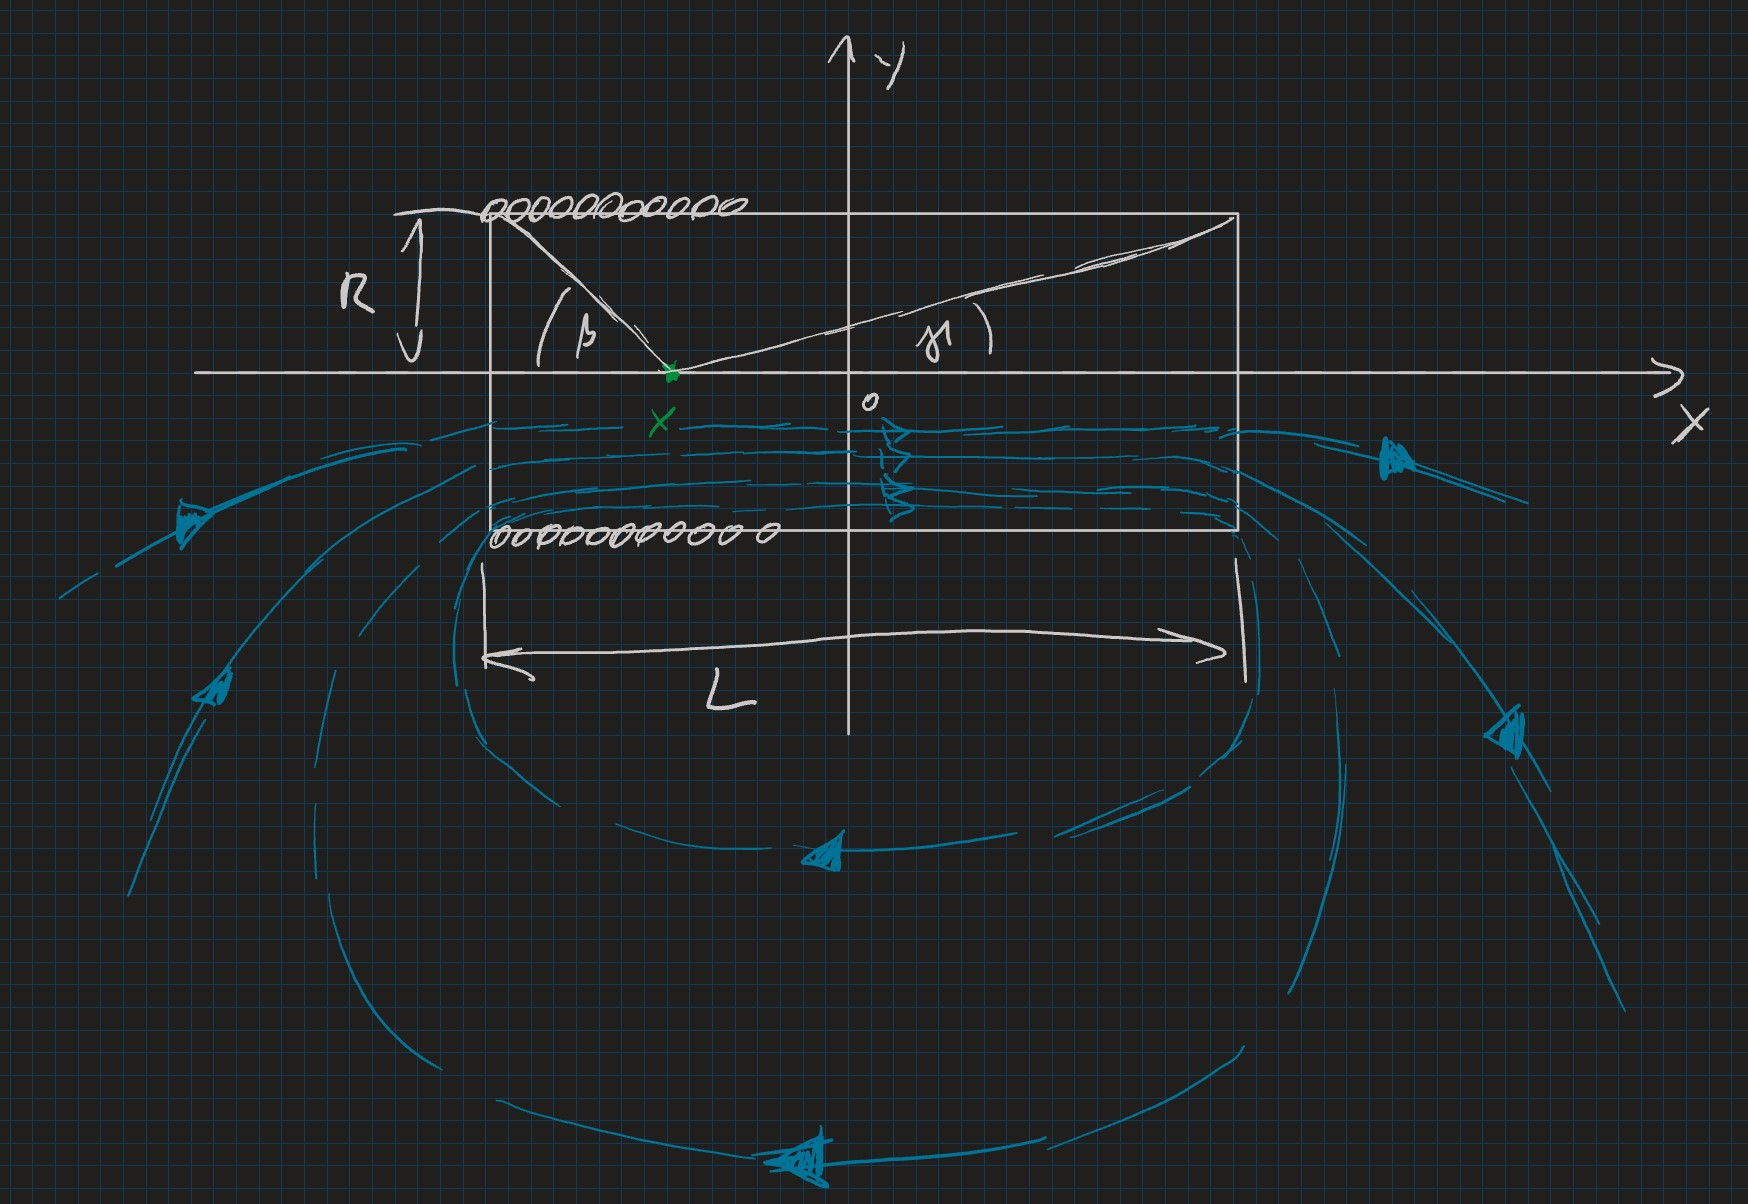
\includegraphics[width=.5\textwidth]{assets/feldInSpule.jpg}
    \label{fig:feldInSpule}
    \caption[Feld innerhalb einer Zylinderspule]{Schematische Darstellung des magnetischen Feldes innerhalb einer Zylinderspule.}
\end{figure}

An der Stelle $ x=0 $ vereinfacht sich \gl{eq:1} zu
\begin{equation}
    H(0) = \frac{I \cdot n}{2} \cdot \left[ \left( \frac{L}{2} \right)^2 + R^2 \right]^{-\frac{1}{2}}
    \label{eq:2}
\end{equation}

Im Falle einer langen Spule ist der Radius im Verhältnis zur Länge als vernachlässigbar klein anzunehmen. Wenn $ R\ll L$
gilt also in guter Näherung

\begin{equation}
    H_{l}(0)    = \frac{I \cdot n}{2} \cdot \left[ \left( \frac{L}{2} \right)^2 + \cancel{R^2} \right]^{-\frac{1}{2}}
                = \frac{I \cdot n}{2} \cdot \left( L \cdot \frac{1}{2} \right)^{-1}
                = \frac{I \cdot n}{L}
    \label{eq:3}
\end{equation}

Kehren sich die Verhältnisse um wird von einer kurzen Spule gesprochen und mit $ R \gg L$ gilt analog
\begin{equation}
    H_{k}(0)    = \frac{I \cdot n}{2} \cdot \left[ \left( \cancel{\frac{L}{2}} \right)^2 + {R^2} \right]^{-\frac{1}{2}}
                = \frac{I \cdot n}{2R}
    \label{eq:4}
\end{equation}
\par\bigskip

Für die Kraft zwischen zwei magn. Polen gilt (analog zur Elektrostatik) \cite{Unbekannt}\cite{Halliday.2005}

\begin{equation}
    F_{mag} = \frac{1}{4\pi \mu_0} \cdot \frac{\phi_1 \cdot \phi_2}{r^2}
    \label{eq:5}
\end{equation}

Ist hierbei $\phi_1$ der Stabmagnet und das Feld innerhalb der Spule mit \(\phi_2 = \vec{B} \bullet \vec{A}\) als vollkommen
homogen angenommen ergibt sich \gl{eq:5} zu

\begin{equation}
    F_{mag} = \phi_1 \cdot H \quad \text{mit} \quad
    H = \frac{1}{4\pi \mu_0} \cdot \frac{\phi_2}{r^2}
    \label{eq:6}
\end{equation}

\begin{figure}[h]
    \centering
    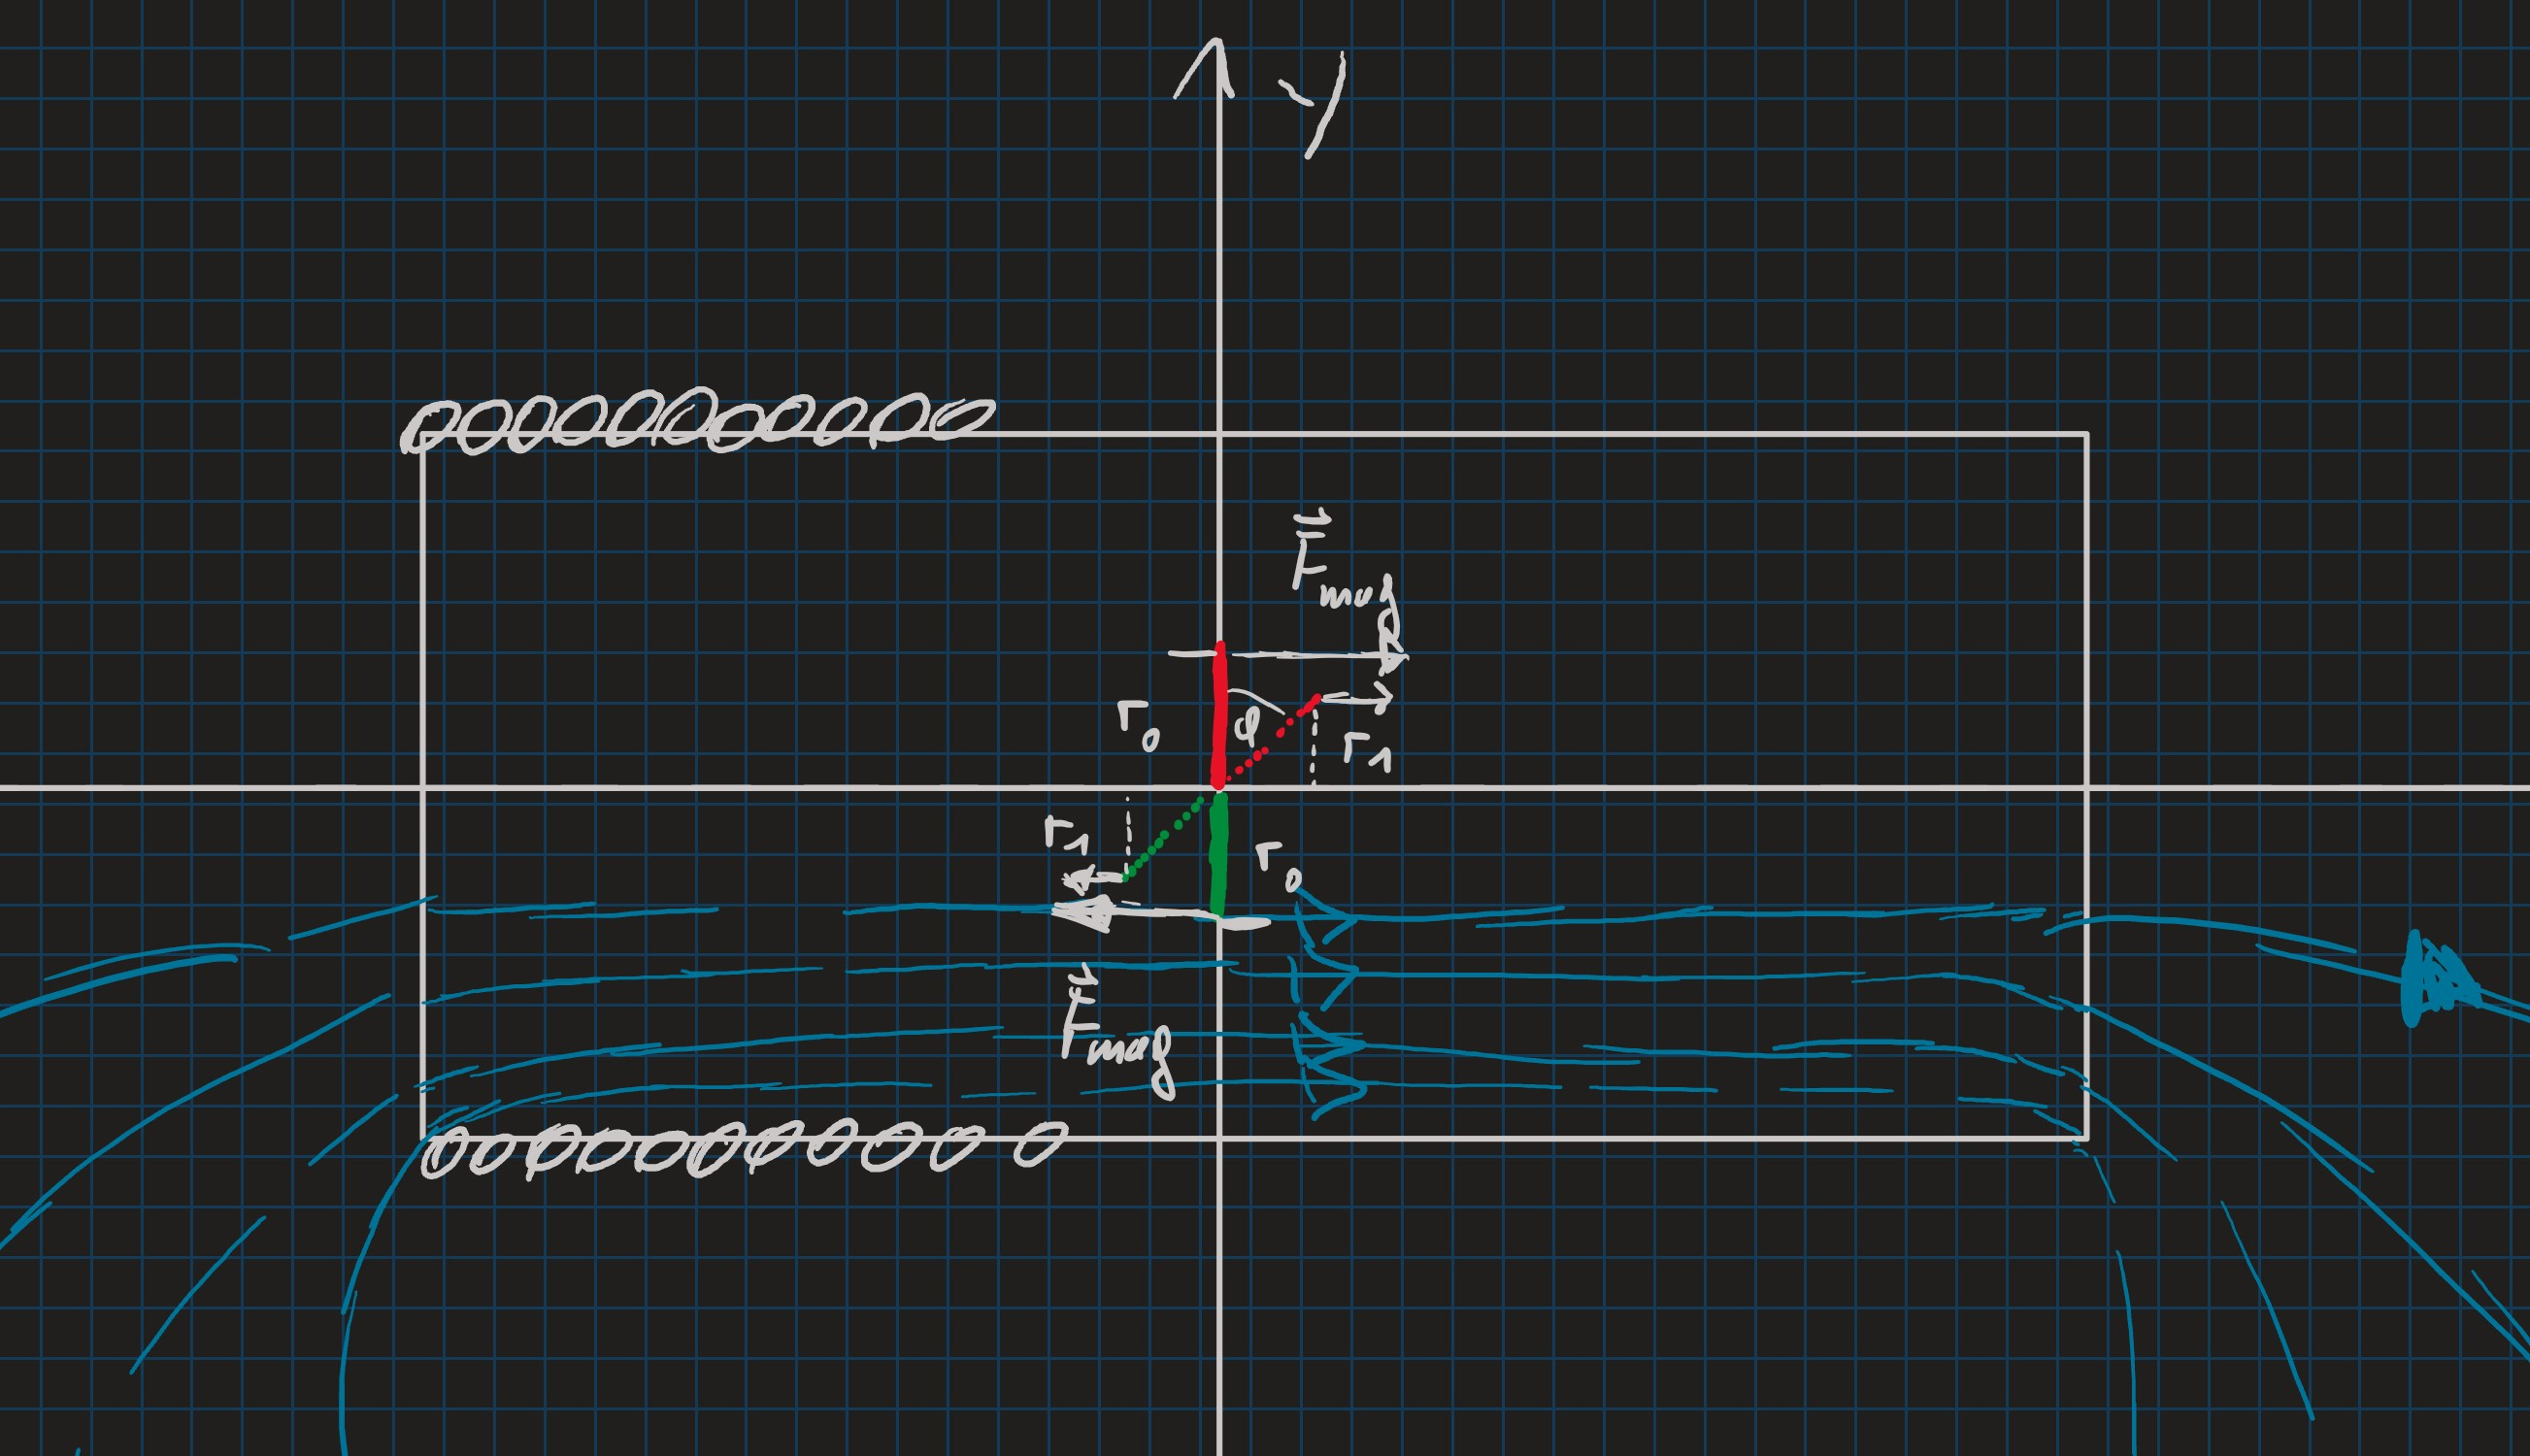
\includegraphics[width=.8\textwidth]{assets/drehmoment.jpg}
    \caption[Kräfte auf einen Stabmagnet im Magnetfeld]{Schematische Darstellung der wirkenden Kräfte auf den Stabmagnet innerhalb der Spule.}
    \label{fig:drehmoment}
\end{figure}
Hiermit und mit $\vec{M} = \vec{r} \times \vec{F}$ lässt sich das auf den Torsionsdraht wirkende Drehmoment ausdrücken durch (vgl. \bild{fig:drehmoment})
\begin{equation}
    M_{mag} = 2 \cdot F_{mag} \cdot r \cdot \cos{\varphi}
    = F_{mag} \cdot s \cdot \cos{\varphi}
    = \phi_1 \cdot H \cdot s \cdot \cos{\varphi}
    \label{eq:7}
\end{equation}
% \par\bigskip

Der Torsionsdraht selbst erzeugt ein umso größeres Rückstellmoment \(M_{Rück} = d \cdot \varphi\), je größer seine Verwindung - also \(\varphi\) - ist.
Ein Kräftgleichgewicht herrscht bei dem Auslenkungswinkel $\varphi$, bei dem die beiden Drehmomente gleich groß sind.
Es folgt durch Gleichsetzen beider Drehmomente und umstellen nach $\varphi$ 
\begin{equation*}
    \phi_1 \cdot H \cdot s \cdot \cos{\varphi} = d \cdot \varphi \quad \Leftrightarrow \quad \varphi = \frac{\phi_1 \cdot H \cdot s \cdot \cos{\varphi}}{d}
\end{equation*}

Unter der Annahme, dass die zu erwartenden Auslenkwinkel ausreichend klein sind verschwindet $\cos{\varphi}$ und es bleibt
\begin{equation}
    \varphi = \frac{\phi_1 \cdot H \cdot s}{d}
    \label{eq:8}
\end{equation}